\newpage
\section{Билет 24. Отказоустойчивость. Активная и пассивная репликация. Алгоритмы поддержания согласованного состояния реплик. Построение надежного хранилища из ненадежных компонентов.}

\begin{center}
	\textit{\underline{Отказоустойчивость}}
\end{center}

\textbf{Отказоустойчивость} — свойство технической системы сохранять свою работоспособность после отказа одной или нескольких её составных частей. Отказоустойчивость определяется количеством единичных отказов составных частей (элементов) системы, после наступления которых сохраняется работоспособность системы в целом. Базовый уровень отказоустойчивости подразумевает защиту от отказа одного любого элемента, однако в теории можно реализовать систему с практическим любым количеством отказов.

Примером отказоустойчивой системы является \href{https://ru.wikipedia.org/wiki/RAID}{RAID}.


\begin{center}
	\textit{\underline{Активная и пассивная репликации}}
\end{center}

В построении отказоустойчивых систем есть два главных подхода к проектированию: активная и пассивная репликация.

\textbf{Активная репликация (на англ. State Machine Approach)} - каждый элемент (реплика) системы хранит копию состояния данных. Операции чтения и модификации выполняются локально в каждом узле. Для поддержания когерентности реплик операции модификации рассылаются всем репликам объекта, которые выполняют их над локальной копией состояния. При выходе из строя части реплик проводится <<голосование>> для выбора реплики, которая будет общаться с клиентом как единственный сервер, поэтому для клиента извне вся система выглядит как один сервер. <<Голосование>> осуществляется с помощью следующих алгоритмов: \href{https://clck.ru/JVS7z}{протокол «Византийского соглашения»}, \nameref{b19:part2}, \href{https://clck.ru/q62LJ}{алгоритм консенсуса}). Отсутствует централизованный контроль, однако в процессе работы выполняется много избыточных вычислений и коммуникаций.
\begin{figure}[H]
	\centering
	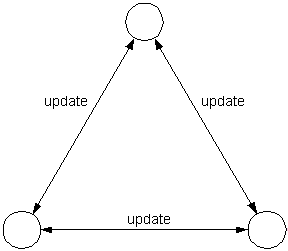
\includegraphics[scale = 0.7]{24/active.png}
	\caption{Схема активной репликации}
	\label{fig:active_repl}
\end{figure}

\textbf{Пассивная репликация (на англ. Primary-Backup Approach)} - каждый элемент (реплика) системы хранит копию состояния данных. Одна из реплик назначается главной. Операции чтения выполняются локально во всех узлах. Операции, модифицирующие состояние объекта, направляются главной реплике, которая, после выполнения метода, обновляет все остальные реплики. При выводе из строя главной реплики пользователь замечает проблемы с доступом к данным, до тех пор пока одна из запасных реплик не возьмет на себя роль главной. Данный метод обладает намного меньшим потреблением ресурсов и отсутствие большого количества избыточных коммуникаций и вычислений в сравнении с активной репликацией, и поэтому используется чаще.
\begin{figure}[H]
	\centering
	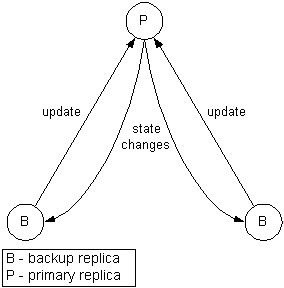
\includegraphics[scale = 0.7]{24/passive.png}
	\caption{Схема пассивной репликации}
	\label{fig:passive_repl}
\end{figure}



	
